\chapter{Mirai static analysis}
\label{chapter:mirai-static-analysis}

In this chapter we delve into the inner workings of Mirai providing a more technical view over its source code. We will go through some of the most important functions and data structures used by Mirai to infect and control IoT devices.

\section{Directory hierarchy}

The original directory hierarchy of Mirai is shown in \Cref{fig:folder-hierarchy}, and it is composed of the following directories: \texttt{dlr}, \texttt{Loader}, \texttt{Mirai} and \texttt{Scripts}. Note that in our repository this structure can be found into \texttt{unmodified\_code} while in order to make the malware running in our environment we had to make some changes to the original code and its structure. 

\begin{figure}[ht]
    \centering
    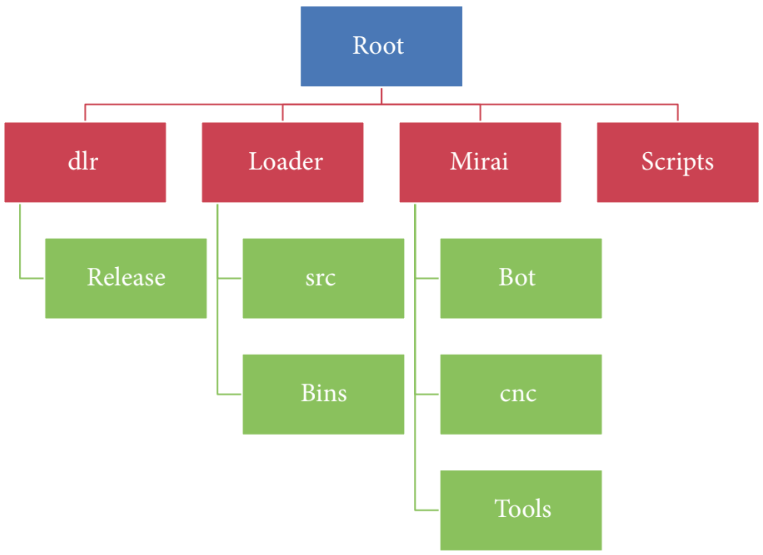
\includegraphics[scale=0.3]{resources/images/folder-structure.png}
    \caption{Original Mirai directory hierarchy \cite{de2018ddos}}
    \label{fig:folder-hierarchy}
\end{figure}

\begin{itemize}
    \item \texttt{dlr}: contains the script needed to compile the \texttt{echoloader} which is a small binary ($\sim$1 KB) that will serve as wget or tftp. The subfolder \texttt{release} contains the echoloader compiled binaries.
    \item \texttt{Loader}: contains the file to execute the loader server. The \texttt{src} subfolder contains its source code and the \texttt{bins} one the binary files of both Mirai malware and the echoloader. 
    \item \texttt{Mirai}: contains the source code of the Mirai malware. This folder is divided into three subfolders:
    \begin{itemize}
        \item \texttt{CNC}: contains the source code of the CNC server written in GO language. 
        \item \texttt{Bot}: contains the source code of the Mirai bots written in C language.
        \item \texttt{Tools}: contains some utility scripts needed to deploy the malware, such as the \texttt{enc.c} script used to encrypt the configuration file and the \texttt{scanListen.go} which implements the Reporting server.
    \end{itemize}
    \item \texttt{Scripts}: contains some utility scripts to compile the malware.
\end{itemize}

Note that the following code snippets are taken from the original Mirai source code, but some part of the code might have been cut out for clarity.

\section{Mirai Scanner}
The Mirai scanner's source code can be found in the `scanner.c' file. The scanner is used by the bots to search for other devices which are potentially vulnerable to the Mirai malware. The search of the devices is performed using random IP addresses generated using the `get\_random\_ip' function. One interesting aspect of this function is that while being random it skips some IP addresses which are reserved for special purposes, such as the internal addresses or reserved ones. In addition to these addresses there are also some standard IPs which are avoided because, according to the comments in the code, belong to special entities e.g. the `Department of Defense' or the `US Postal Service'. The complete list can be found in Figure~\ref{fig:random_ip}. Instead of performing an entire telnet handshake to check the validity of an IP address the bot sends a TCP SYN packet and if the response it gets is a SYN+ACK packet it starts a dictionary attack against the host. The dictionary is composed of ~60 credentials which are known to be used as default ones (e.g. admin:admin, root:root), all the entries are encrypted to make the reverse engineering harder. More details on the encryption algorithm are provided in Section~\ref{section:ex1}. To handle the possible state transitions of the telnet interaction a switch statement that works as a state machine is used~\cite{de2018ddos}. Once a valid credential is found the bot sends the information to the reporting server which will share it with the loader server. The scanner is also able to detect if the device is already infected by checking if the device is listening on port 48101. If the device is already infected the bot will not try to infect it again~\cite{mirai-hackforum}.

\begin{figure}[ht]
    \centering
    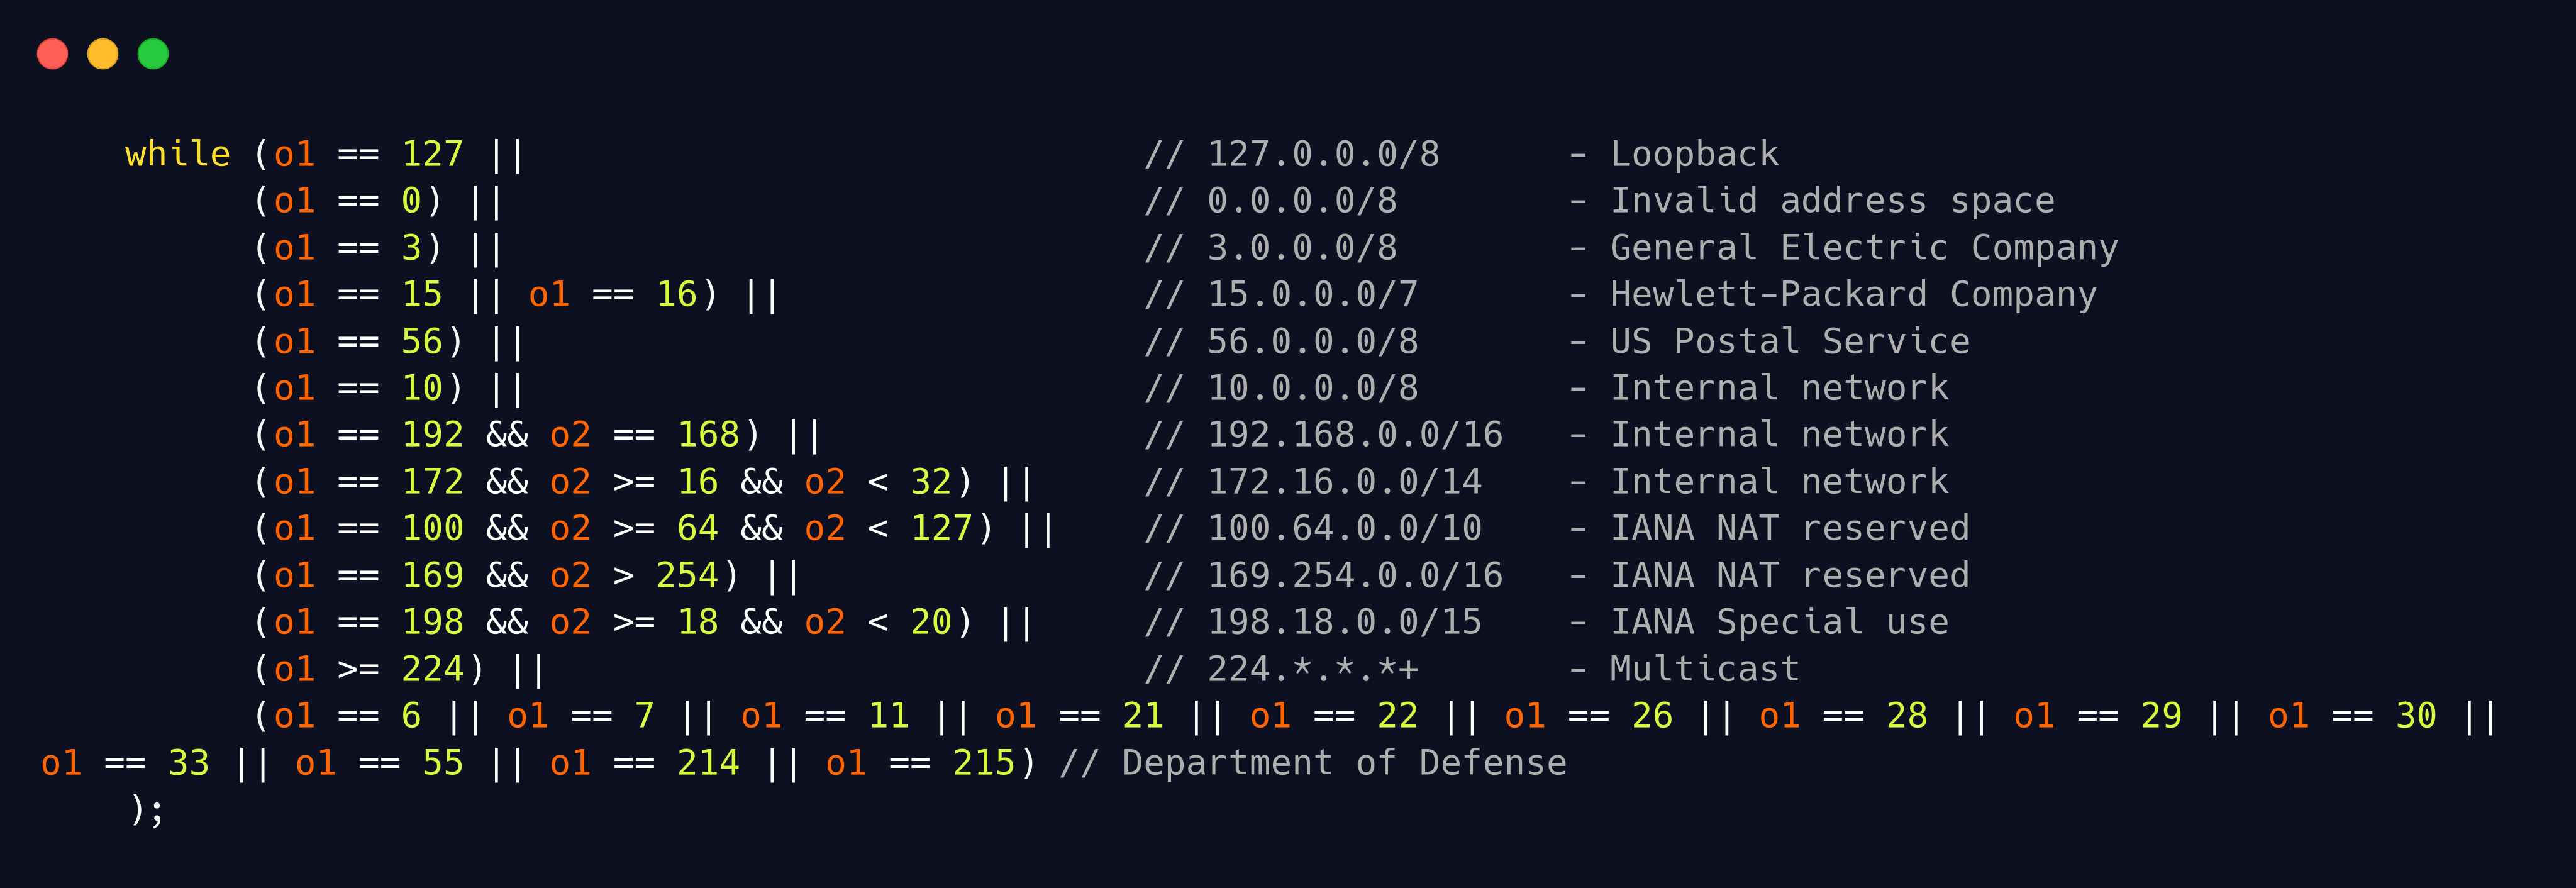
\includegraphics[scale=0.12]{resources/images/get_random_ip.png}
    \caption{Whitelisted IPs in get\_random\_ip function}
    \label{fig:random_ip}
\end{figure}

\section{Loader server}

As we said in \Cref{chapter:introduction} the \textbf{Loader server} is in charge of receiving the vulnerabilities from the Reporting server and use them to load the malware on the reported devices. The vulnerabilities received must be in the following format:

\[ \text{\texttt{ip:port} \texttt{user:pass}} \]

The Loader has three main components:
\begin{itemize}
    \item \textbf{Pool of workers}: a worker is a thread whose job is to process the received vulnerabilities and infect the devices. 
    \item \textbf{List of vulnerabilities}: list of information that can be used to access the insecure devices. 
    \item \textbf{Binary source code}: cross-compiled binary for different architectures. 
\end{itemize}

The source code of the loader is into the \texttt{loader/src} folder. The entry point is the \texttt{main.c} file where all the needed data structures are initialized and it has two main parts:

\begin{itemize}
    \item The \texttt{server\_create} function which is illustrated in \Cref{fig:server-create}. It takes as input the \textbf{numbers of workers} to create and both the \textbf{IP address} and \textbf{port} for \textbf{wget} and \textbf{tftp}.
    \item Then it starts \textbf{listening} for incoming reports from the Reporting server. When a report is received, it calls the \texttt{server\_queue\_telnet} function which checks if maximum number of connection (variable \texttt{max\_open}) has been reached. If not, it invokes \texttt{server\_telnet\_probe}. This is shown in \Cref{fig:mainloop}.
\end{itemize}

\begin{figure}[ht]
    \centering
    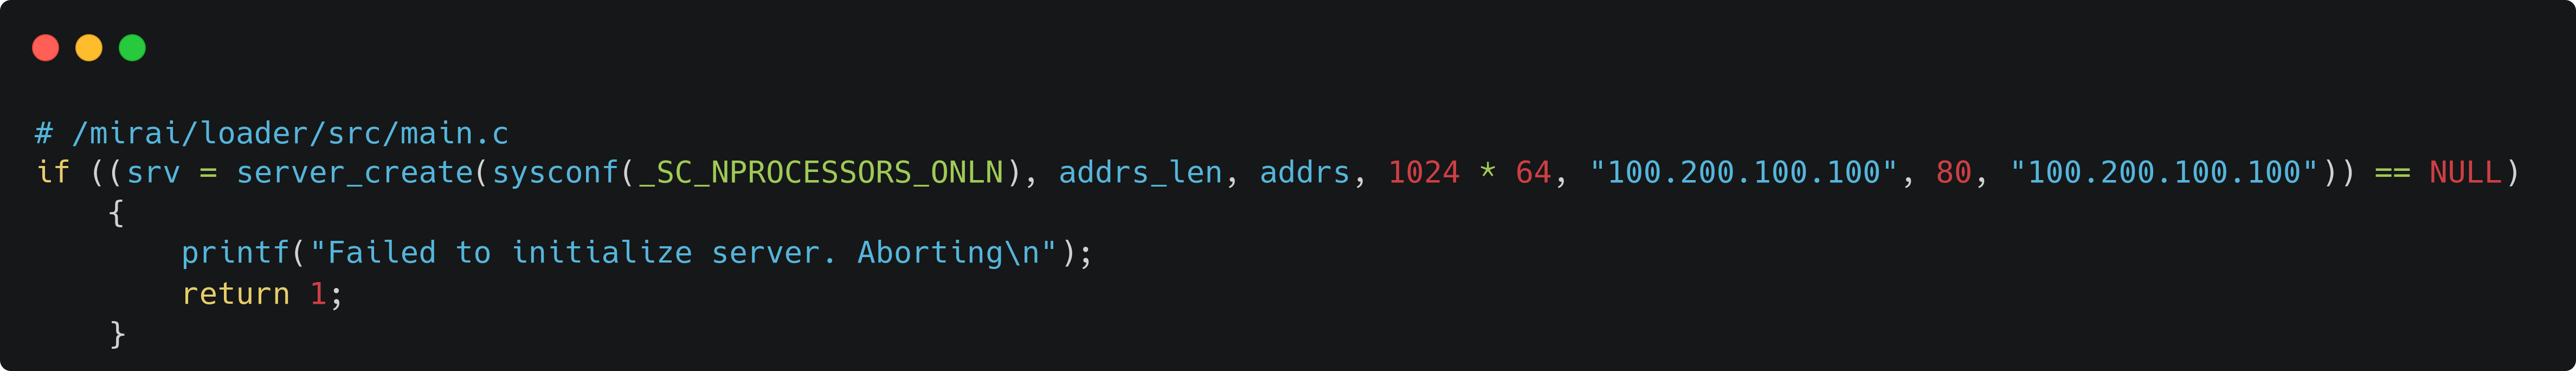
\includegraphics[scale=0.1]{resources/images/server_create.png}
    \caption{\texttt{server\_create} function}
    \label{fig:server-create}
\end{figure}

\begin{figure}[ht]
    \centering
    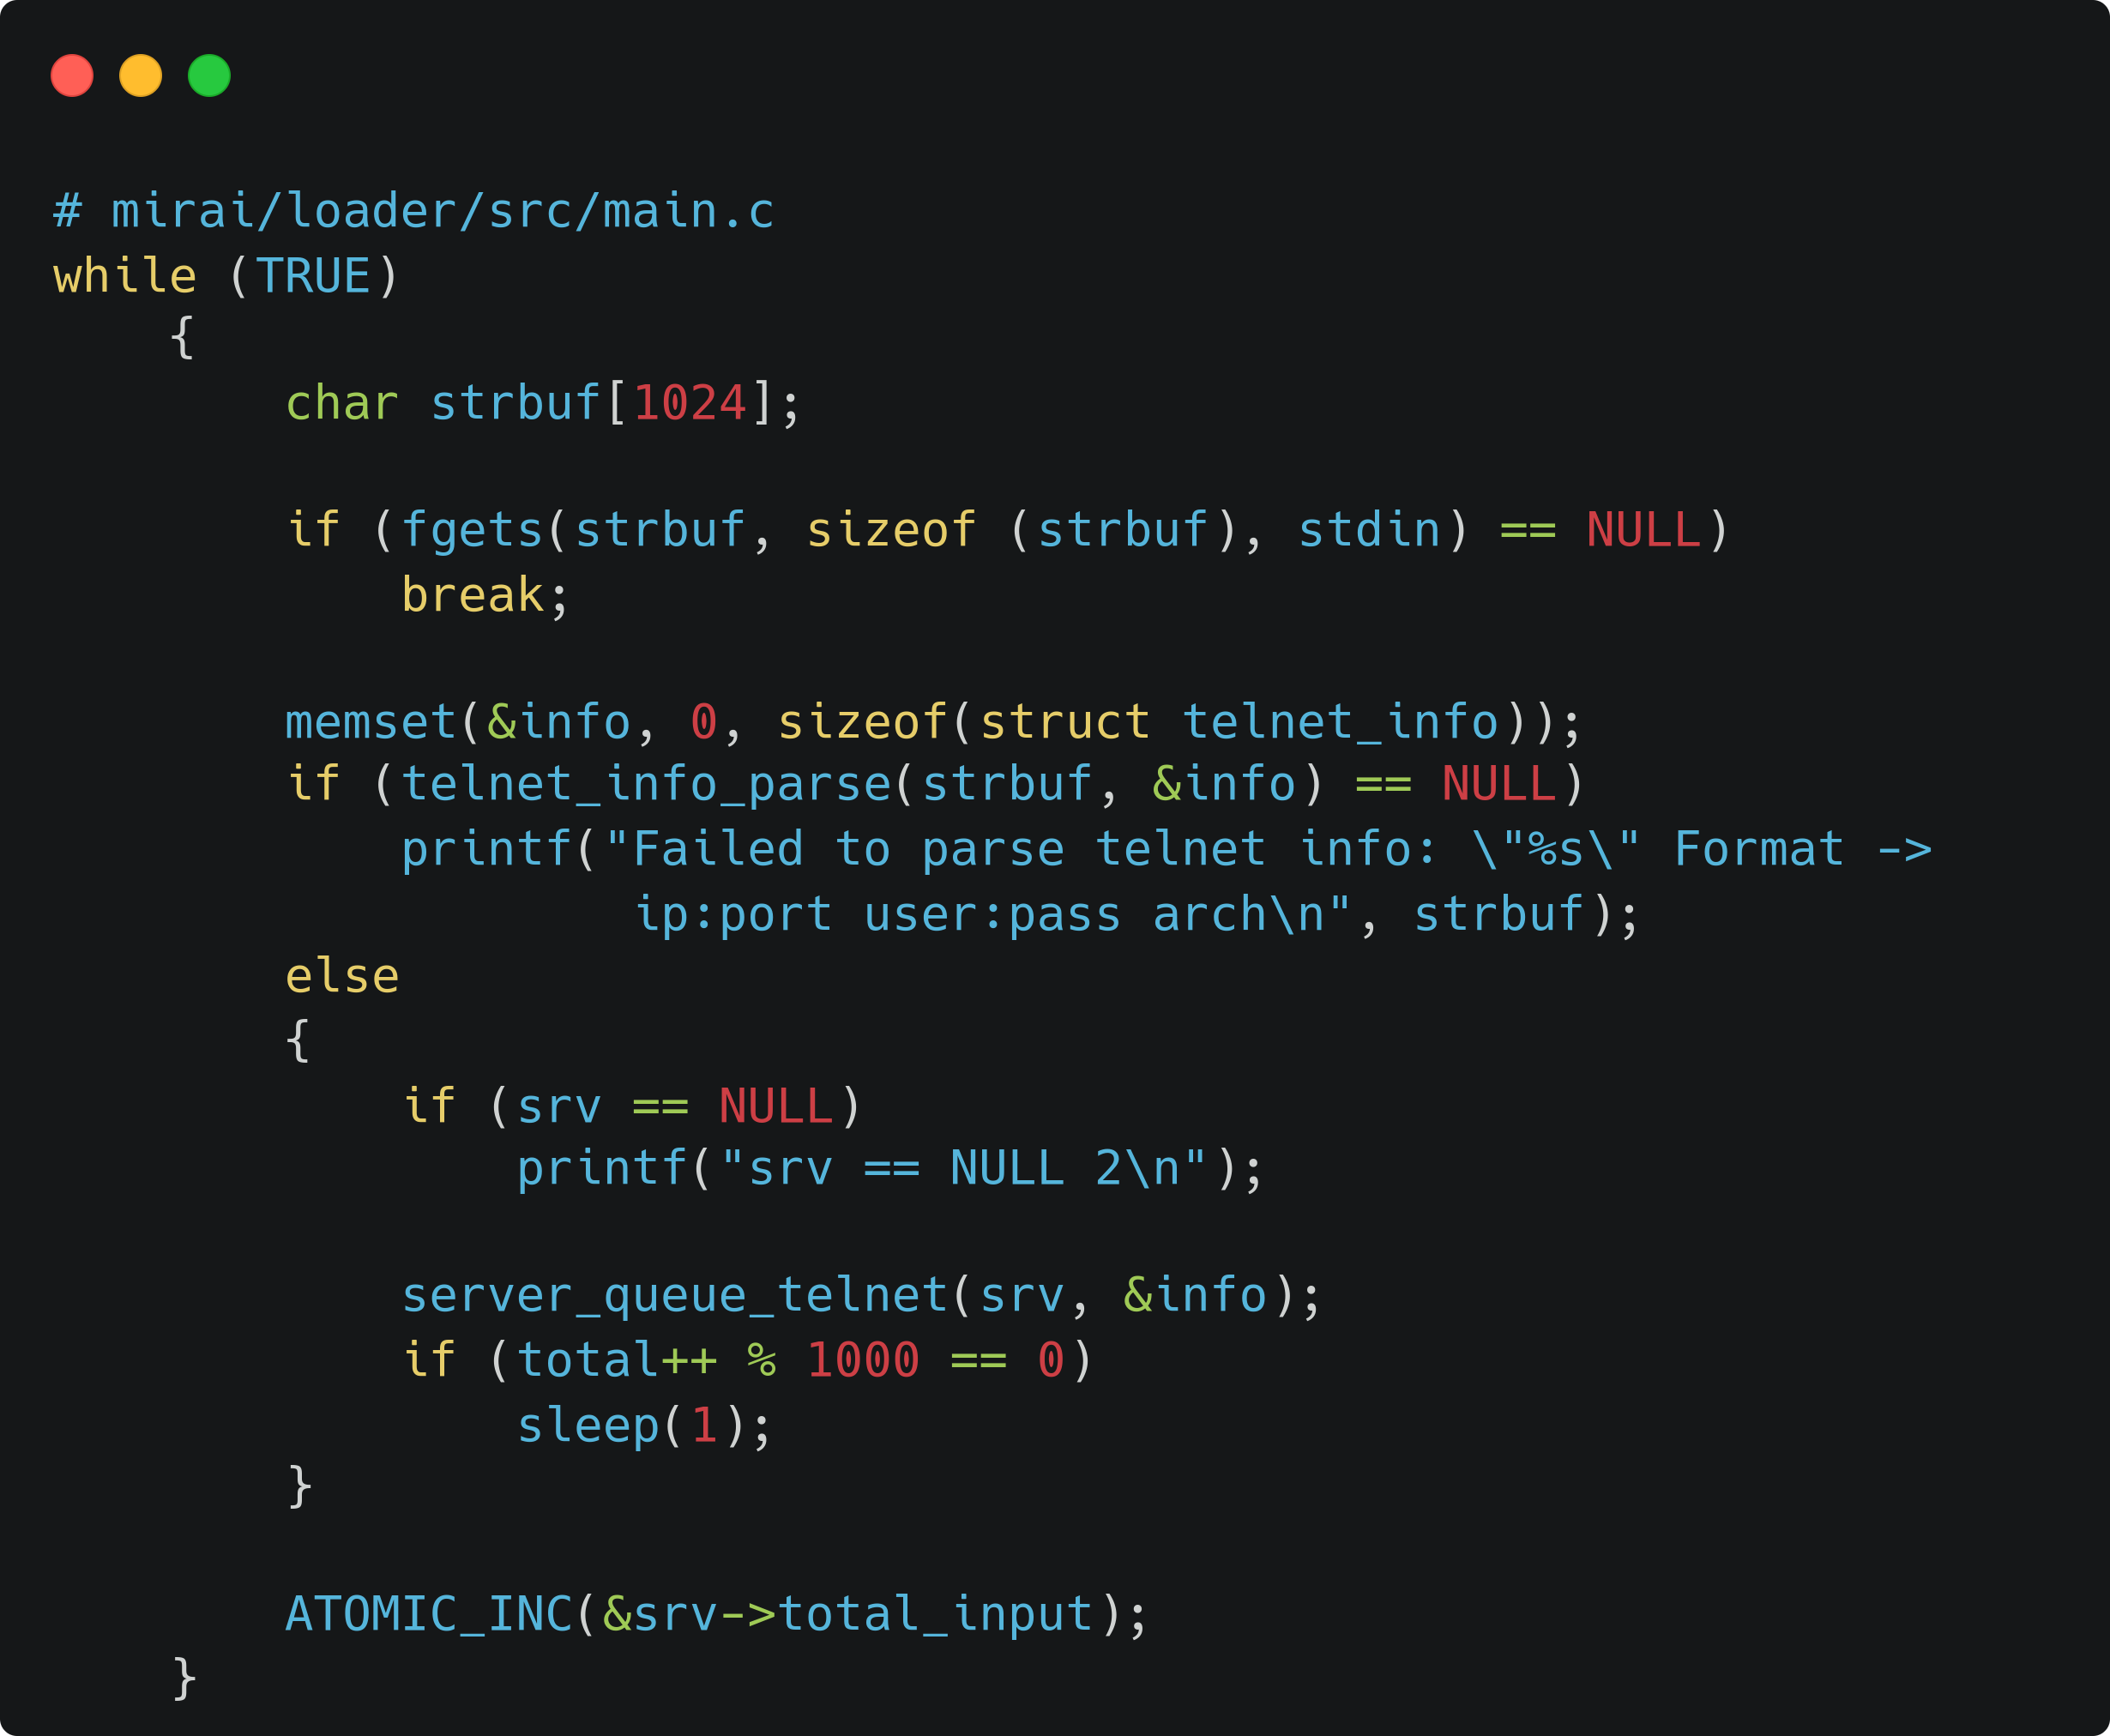
\includegraphics[scale=0.1]{resources/images/main.png}
    \caption{\texttt{main.c} loop}
    \label{fig:mainloop}
\end{figure}

The \texttt{server\_telnet\_probe} is shown in \Cref{fig:server-telnet-probe}. Its role is to \textbf{set up a connection} with the remote device and \textbf{cyclically} add new \textbf{event} to the epoll of the selected worker. In this way as soon as a worker is free, it will be able to call \texttt{handle\_event}.

\begin{figure}[ht]
    \centering
    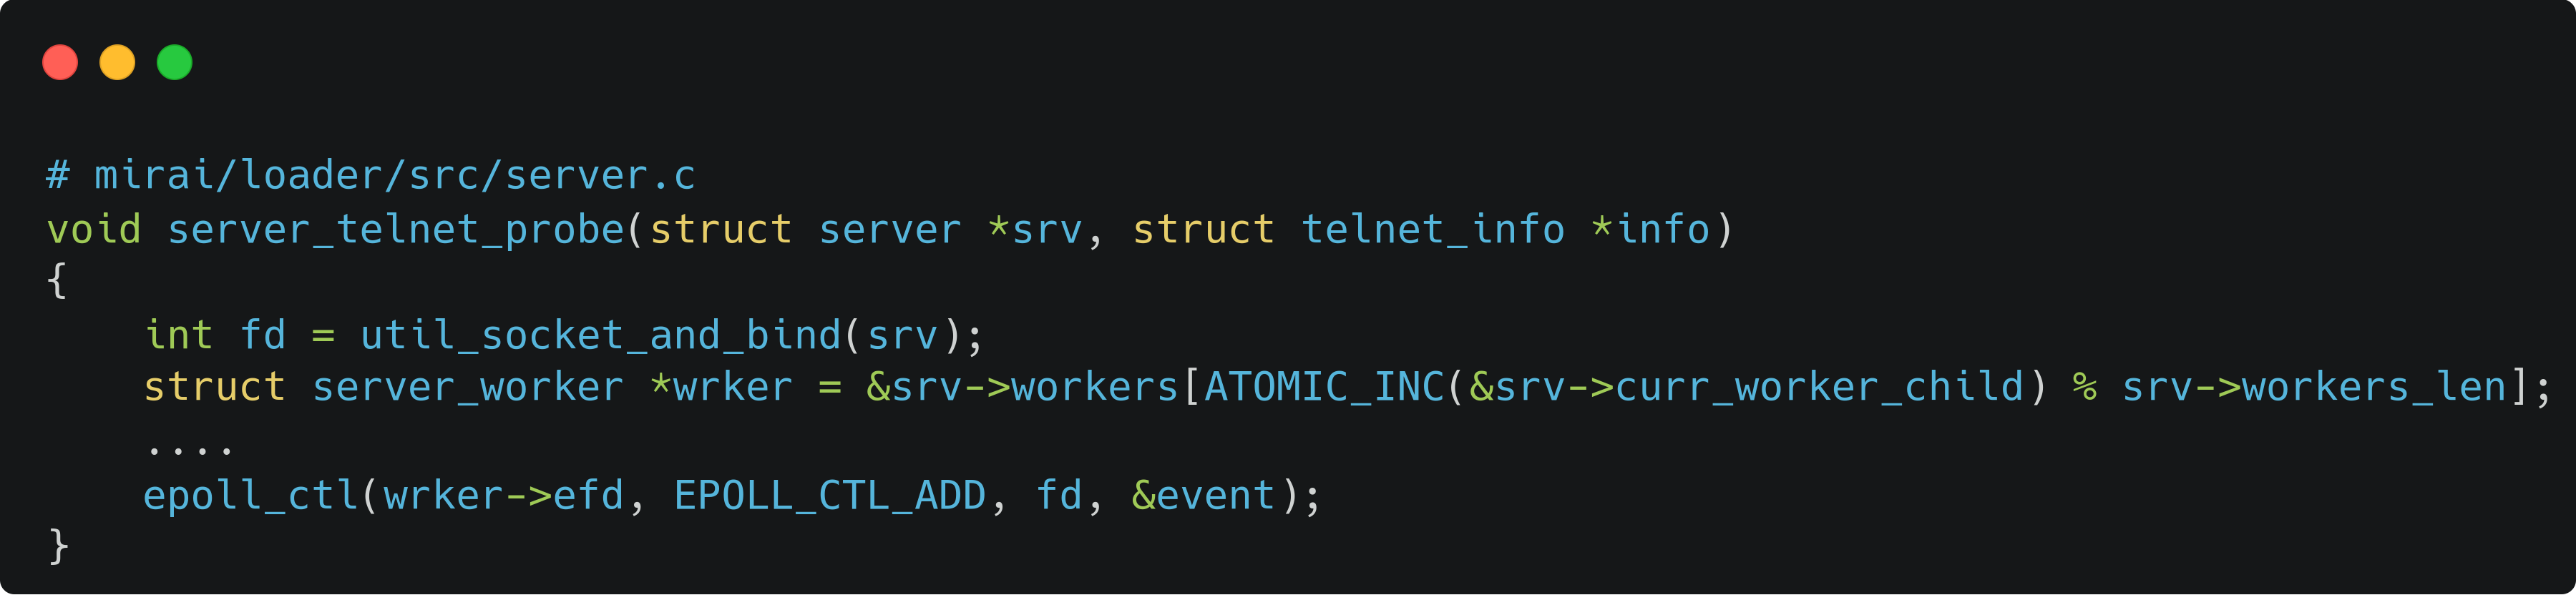
\includegraphics[scale=0.15]{resources/images/sever_telnet_probe.png}
    \caption{\texttt{server\_telnet\_probe} function}
    \label{fig:server-telnet-probe}
\end{figure}

Since the source code of the \texttt{handle\_event} is quite long, we will not show it here. Its role is to interact with the remote device using a switch statement that performs \textbf{various actions} based on a \textbf{state machine}, which is shown in a simplified way in \Cref{fig:state-machine}

\begin{figure}[ht]
    \centering
    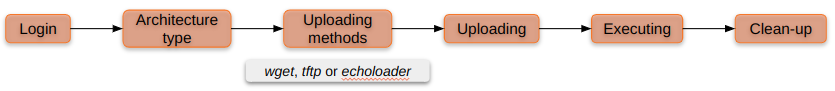
\includegraphics[scale=0.5]{resources/images/state-machine.png}
    \caption{State machine of the \texttt{handle\_event} function}
    \label{fig:state-machine}
\end{figure}

What we have said so far, can be summarized as follow: when a vulnerability result is received, it is added to a worker's list of vulnerabilities. All workers are actively waiting for elements in their lists to process. Once a vulnerability is available, a worker uses the information to access a weak device. It then identifies the device's architecture to load the appropriate executable. The worker tries to upload the binary code to the device using either wget or tftp . If neither is available, the ``echoloader'', which functions similarly to wget, is loaded onto the victim using the Linux echo command and is then used to upload the worm binary code. Once uploaded, it is executed and the device is turned into a Mirai bot.\cite{de2018ddos}